\section{Introduction}
\label{sec:intro}

Writing a Geant4\cite{geant4} simulation that read volumes definitions from a database is
as easy as replacing calls like \verb|G4Box(‘box’, 20, 30, 40)| with
\verb|G4Box(name, a, b, c)| where the parameters are read from a database.
This however is not particularly useful: users still write c++ and geant4 code to setup
the volumes definitions organization, sensitivity, how to digitized the geant4 steps
and collect them into hits saved in some output format.

\begin{figure}[h]

    \centering
    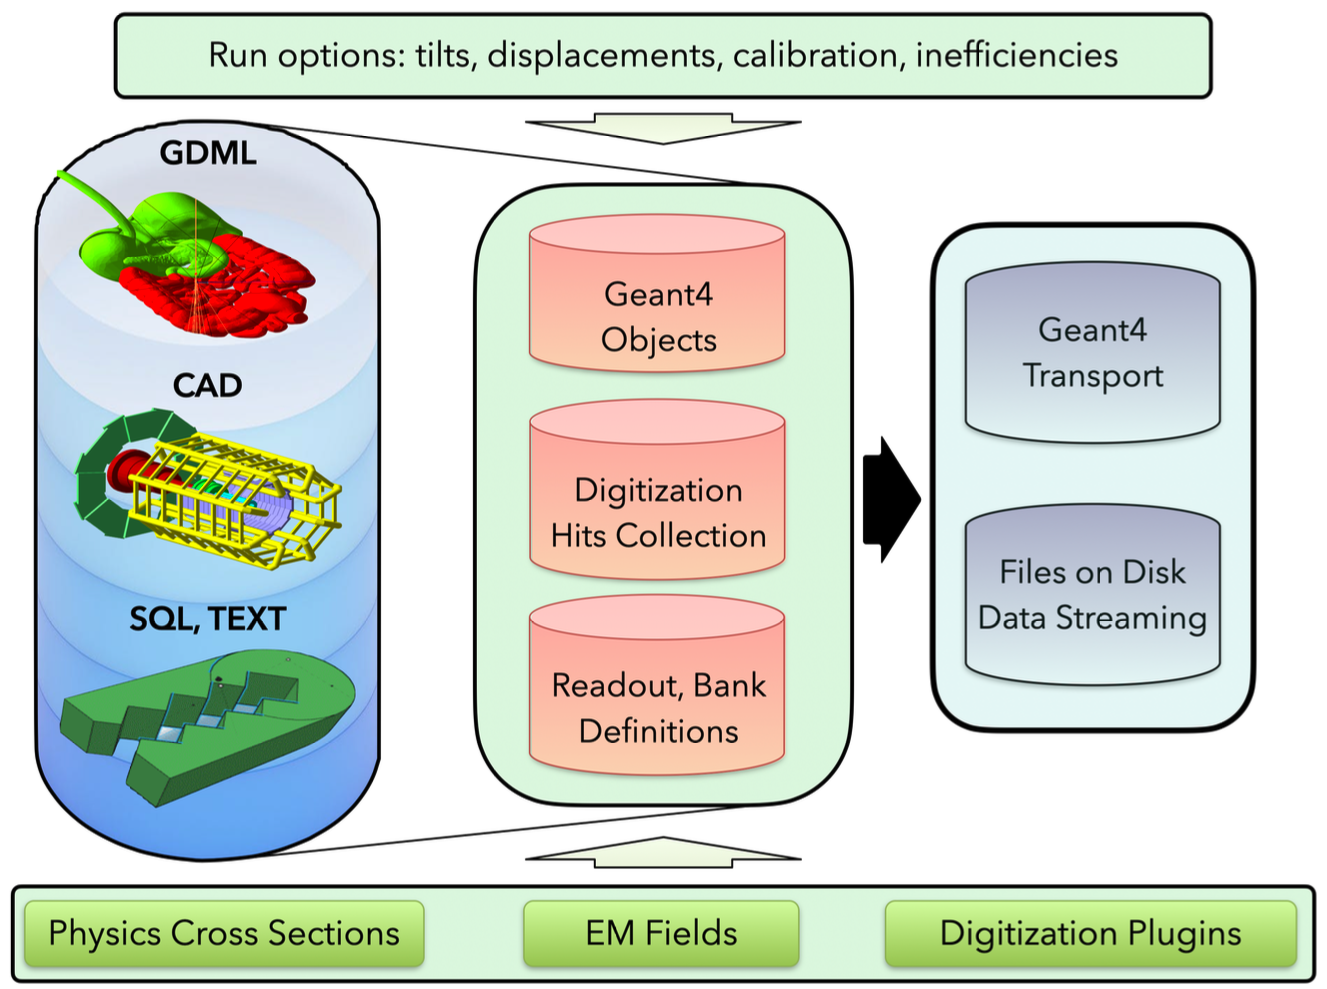
\includegraphics[width=1cm,clip]{img/db}
    \caption{A geant4 application driven in its entirety by a database: geometry, materials,
        digitization, readout electronics, output format.}
    \label{fig:db}
\end{figure}

Far more useful would be the application sketched Fig.\ref{fig:db}, capable of defining, in its entirety, an
experiment setup simulation from a database:


\begin{itemize}
    \item the experiment setup is defined in a single place, the database, and can be
    modified without recompiling the code
    \item the experiment setup can be shared among different users
    \item the same application can be used to simulate different experiments, by simply
    selecting the desired setup from the database
    \item no pre-requisite knowledge of c++ or geant4 required to write the simulation
\end{itemize}

GEMC\cite{clas12_gemc} is a such an application.
Stemming from 20 years of experience of the Jefferson Lab Hall B software group
on detector design, simulation, detector calibration, data reconstruction and processing,
it provides:

\begin{itemize}
    \item a python API to build detectors and populate the databases
    \item hardware emulation of the readout electronics
    \item energy sharing mechanism
    \item user defined digitization of the geant4 steps
    \item data streaming to disk or network
\end{itemize}


\section{Features}
\label{sec:features}

\subsection{Databases}
\label{subsec:databases}

\subsection{Python API}
\label{subsec:api}

\subsection{Electronic Time Window}
\label{subsec:time_window}

\subsection{Energy Sharing}
\label{subsec:energy_sharing}

\subsection{Digitization}
\label{subsec:digitization}

\subsection{Data Streamer}
\label{subsec:data_streamer}


\section{Examples}
\label{sec:examples}

\subsection{Cad Import}
\label{subsec:cad_import}

\subsection{Flux scintillator paddle}
\label{subsec:flux_scintillator_paddle}

\subsection{GEMC at Jefferson Lab}
\label{subsec:clas12}


\section{Summary}
\label{sec:summary}

